\documentclass[10pt, oneside,onecolumn]{IEEEtran}

\usepackage{geometry} 
\usepackage{listings}
\usepackage{xcolor}

\usepackage[colorlinks = true,
            linkcolor = blue,
            urlcolor  = blue,
            citecolor = blue,
            anchorcolor = blue]{hyperref}
            
\definecolor{bluekeywords}{rgb}{0,0,1}
\definecolor{greencomments}{rgb}{0,0.5,0}
\definecolor{redstrings}{rgb}{0.64,0.08,0.08}
\definecolor{xmlcomments}{rgb}{0.5,0.5,0.5}
\definecolor{types}{rgb}{0.17,0.57,0.68}

\usepackage{listings}
\lstset{language=[GNU]C++,
commentstyle=\color{greencomments},
morekeywords={partial, var, value, get, set},
keywordstyle=\color{bluekeywords},
stringstyle=\color{redstrings},
}
\lstset{language=Python,
morekeywords={partial, var, value, get, set},
keywordstyle=\color{greencomments},
stringstyle=\color{types},
}

\usepackage{graphicx}  
\usepackage{float}
\usepackage{caption}             		
\geometry{letterpaper, margin=.75in}                   		
\usepackage{graphicx}										
\usepackage{amssymb}
\usepackage{indentfirst}
\usepackage{courier}	
\usepackage[section]{placeins}

\begin{document}

\setcounter{tocdepth}{0}
\tableofcontents

\begin{titlepage}
\begin{center}
        \vspace*{6cm}
        {\Huge Mars Rover Navigation}\\[1cm]
        {\Large Team 21: Jay Fenton, Alexander Arreguin, Ian Riemer}\\[.5cm]
        {\Large CS 463 Senior Capstone}\\[.5cm]
        {\Large Spring Term}\\[.5cm]
        {\Large June 10th 2016}\\[8cm]
\end{center}

%{\normalsize This document presents capstone team 21's work on the Oregon State Mars rover navigation and avoidance software. The rover has been entered in The Sample Return Robot Challenge, a university robotics competition hosted by NASA. The final software allows the rover to efficiently navigate unknown terrain by using sensor input to avoid obstacles and recognize a base station which it maneuvers back to. The navigation system integrates with other software systems present on the rover.}\\[2cm]
\end{titlepage}

\section{Introduction}

An introduction to the project.

STILL NEED:
What is its importance? -kinda stated
Who are the members of your team?
What were their roles?
Project Purposes and Goals


\subsection{Our Client}

The president of the Mars Rover team, Billy Edwards, requested two software capstone teams to help develop the autonomous programs for the rover. The Sample and Return Robot Challenge, which the rover team participates in annually, requires that rovers run sophisticated software to complete levels of the challenge. In previous years the volunteers on the team had struggled with creating software capable of completing levels. Billy wanted dedicated senior capstone teams to create the software for the 2016 competition. Our teams responsibility was to develop the automated navigation and avoidance routines for the rover. 

Billy had a very active role in overseeing our project. Along with handling all the team administration responsibilities, he helped design the mechanical components on the rover. We met with Billy at least once a week for Fall and Winter terms in official meetings, and multiple times a week Spring term in the Robotics Club lab where we worked on the project. 

\subsection{Project Overview and Importance}

The Sample Return Rover Challenge is a NASA Centennial competition. The Centennial Challenges were designed to let citizens participate in solving challenging problems by providing many diverse solutions to the problem. This rover challenge requires teams to autonomously retrieve samples and deliver them back to a base station where the rover started from. Rovers entered must adhere to a set of rules that simulate conditions on Mars. Earth based sensors such as global positioning systems (GPS) and magnetic compasses are not allowed. Teams may not communicate with their rovers while the rover is on the course. The competition is split into two levels, and teams must complete level one successfully to compete in level two. 

\subsection{Competition Details}

Level one requires teams to pick up a known pre-cached sample as well as an easy sample, and will take place from the 6th-11th of June 2016. The pre-cached sample is a nylon cylinder with a metal hook. The easy sample will be a rock painted within a known HSV (hue, saturation, value) range and 10-12 cm in diameter. We know that the terrain will be one quarter of a football field. The locations of the two samples we must collect have been provided, along with the base station location. It was required that teams submit a video by April 8, 2016 to participate in level one. The retrieval video can be found on the robotics club \href{https://www.youtube.com/watch?v=H8sDekAOodg}{Youtube channel}.

Level two requires teams to pick up various colored rock samples and metal objects. Coordinate locations and radii that indicate areas in where a sample may be placed have been provided to us. Although these points define regions of interest, we are given 15 points and know only six samples, the easy and medium samples, correspond to those locations. Medium samples will be rocks painted in a more broad HSV range than the easy samples, and are 6-8 cm in diameter. There are also hard samples on the field which do not have a known region associated with them. The hard samples are metallic non-ferrous objects 5-10 cm in diameter that have a marking on them. We know the course is in a park, and the topography is provided which gives us an idea of the type of terrain and obstacles that we may encounter. Sample groupings have corresponding point values, the more samples collected the more points a team may get. For a team to earn their points the rover must return the to the base station it started at. Level two will take place from the 2nd-5th of September 2016.

\subsection{Team Members and Roles}
The three members of team 21 were Jay Fenton, Alexander Arreguin, and Ian Riemer. 

\subsection{Project Purposes and Goals}

The goal of our project was to develop an autonomous navigation system for the rover that integrated with the other systems present. This included the Uniboard API which was written by the electrical team to interface with the hardware, the sample collection code that the other


\section{Requirements Document}

\subsection{Introduction}

\subsubsection{Purpose}
This document provides an outline of project requirements for the navigation and object avoidance software system to be designed for the Oregon State University Mars Rover. Intended readers are those who are overseeing the project as well as members of other teams who are working on the project 

\subsubsection{Project Scope}
The focus of this project is to identify and select the most capable depth sensing technologies that can be affordably mounted to the OSU Mars Rover and to develop software that will process the information from the sensors to navigate the rover. The OSU Mars Rover Navigation and Avoidance Software must be able to maneuver the rover around a given challenge field, identify potential obstacles for the rover, and respond to the obstacles by maneuvering the rover around them. The rover will navigate to known locations search for objects, and navigate the to a base station once the mission is over. 

The Rover Navigation and Avoidance Software will not need to specifically identify whether an object is an objective or an obstacle, though it may alert the Object Recognition Software if the object matches certain criteria that might indicate an objective, such as meeting certain dimensions or color specification. The navigation software will run as a state on the rover, where it remains in the navigation state until a condition triggers another state to take over, such as the object pick-up state. The software needs to be able to maintain its understanding of the rover's location while it is in other states. The software does not need to guide the rover to pick up an object once the Object Recognition Software has an objective sample; the movements of the rover will be controlled by its current state. 

\subsubsection{Project Overview}
The team will develop the autonomous navigation system for the Oregon State University Mars Rover. The rover will be competing in The Sample Return Robot Challenge, a university robotics competition hosted by NASA. The software developed will allow the rover to efficiently navigate unknown terrain by avoiding obstacles and recognizing a base station that it will be able to maneuver back to. The navigation system will integrate with other software systems present on the rover. 

\subsubsection{Competition Overview}
In The Sample Return Robot Challenge, teams build and enter rovers that will autonomously navigate a course and collect and return as many samples as possible to a base station. The competition is split into two distinct phases. 
The first level requires teams to navigate and retrieve two samples, one pre-cached sample and one easy sample. The exact pre-cached sample location is known, along with the exact shape and color. The easy sample is a painted rock placed within a known region. We currently do not know the terrain for level 1, however given the rules some Rover club members believe this may take place on a football field.

To compete in level 2, level 1 must be successfully completed. In level 2 we seek easy, medium, and hard samples. The locations of these samples are not known, however the general area samples are located in will be giving to us in early January along with a contour map of the terrain we must traverse. The easy and medium samples are various sized painted rocks, while the hard samples are non-ferrous metal objects with a logo imprinted on them. 

\subsection{Description}
\subsubsection{Product perspective}

\begin{figure}[H]
\centering
\includegraphics[width=170mm]{Navigation_Block_Diagram.eps}
\caption{Navigation Block Diagram}
\end{figure}

\begin{figure}[H]
\centering
\includegraphics[width=170mm]{Avoidance_Block_Diagram.eps}
\caption{Avoidance Block Diagram}
\end{figure}

\begin{figure}[H]
\centering
\includegraphics[width=170mm]{Return_to_Home_Block_Diagram.eps}
\caption{Return to Home Base Block Diagram}
\end{figure}

\subsubsection{Product functions}
	The functions the software will perform fall into two categories, navigation and avoidance. The navigation functions will work to move the rover towards a target location, based on the areas of interest provided in the contour map. As the rover moves towards a location, sensor input will be analyzed to gather information about the rover's position. If obstacles are discovered that must to be avoided the rover will transition into the avoidance functions. During the navigation routine the rover will periodically check if it needs to return to the home base. This return may be signaled by a timer or by a total number of samples collected.  
	When the avoidance function is triggered the rover will determine how it should avoid the obstacle. The avoidance routine will maneuver the rover around the obstacle and to a location where it may resume navigation toward the planned location. After the routine ends, the rover will do a self-check and determine if it has in fact avoided the obstacle. During navigation, interrupts are expected from the object recognition software system. When this occurs the rover will pause on it?s current path and allow for the object recognition software to provide an updated location to travel towards if an object is located. 

\subsubsection{Constraints}
The constraints on this project come from the rules of the competition and the mechanical and electrical systems on the rover. The rover may not use sensors that rely on earth's magnetic field or earth-orbit based radio aids. Additionally, communication with the base station must use technology that complies with FAA regulations. Other software constraints include processing and power usage, which limits the amount of cameras we can use. To qualify for level one a video must be submitted of the rover completing the sample collection 30 days prior to the event. To meet this deadline the software will need to be working and tested in early April. 

\subsubsection{Assumptions and dependencies}
The navigation and avoidance software must be tested thoroughly. The team assumes that the bulk of the software development will take place in winter term and the testing will take place alongside development and through spring term. This plan depends on the mechanical and electrical teams getting their parts of the project done quickly. Although development may take place while the rover is undergoing mechanical and electrical changes, to test and improve the navigation and avoidance system, the rover should be fully functioning. 

\subsubsection{Functional Requirements}
The rover shall do the following:
\begin{enumerate}
\item Scan and interpret the environment to know the surroundings
\subitem Use LIDAR, Infrared depth cameras, and/or a stereoscopic camera system to gather information
\subitem Use SLAM or another mapping algorithm, the software will map the rover's path

\item Navigation routine will avoid obstacles 
\subitem Differentiate between wall and hills
\subitem Move the rover within the boundaries of the course
\subitem Allow the rover to return back to the base station

\item The software can determine robot's position to estimate the following
\subitem Distance from the base
\subitem Distance from the obstacles 
\subitem Distance from the samples
	
\item The rover completes level 1 by completing the following
\subitem Picks up the pre-cached sample and one easy sample
\subitem Returns to home base with both objects
\subitem Completed in under 30 minutes

\item Camera sensing requirements 								
\subitem Field of View: minimum of 90 degrees 
\subitem Resolution: 480p
\subitem FPS: at least 30
\end{enumerate}


STILL NEED: Gant Chart

\section{Project Changes}

How did the project change since the original Client Requirements Document?
What new requirements were added? What existing requirements were changed? What existing requirements were deleted? Why?
Use the following table format:

What was the final Gantt chart?

\section{Design Document}

\subsection{Introduction}

\subsubsection{Challenge and Project Overview}

The Navigation and Avoidance Trio (NAT) will develop an autonomous navigation system for the Oregon State University Mars Rover. The rover will be competing in the NASA Sample Return Robot Challenge, a university robotics competition. The rover team's entry proposal is due in January, 2016. The competition is split into two levels. Level 1 of the competition requires teams to pick up a known sample as well as an unknown sample. Locations of the samples are provided. Level 1 will take place on the 6th-11th of June 2016. To participate in level 1, a video must be provided one month prior to the competition date showing completion of sample retrieval. Level 2 requires teams to pick up various colored rock samples and metal objects. The general areas some samples are placed in are provided. Level 2 will take place on the 2nd-5th of September 2016. The software developed by NAT will use sensor input to direct the rover and navigate unknown terrain by, avoiding obstacles it encounters. The rover will also recognize a base station which it will be able to maneuver back to. The navigation system will integrate with other software systems on the rover.

\subsubsection{Date of Issue and Status}

This project was issued on 4 Oct 2015. Plans and schedules for development have been created but development has not yet begun. It has been decided which tools will used for the navigation system including sensors, operating system, programming languages. An plan of how the navigation software will interact with the other software on the rover has been developed. 

%\subsubsection{Project Timeline}

\begin{table}[H]
\centering
\caption{Project Timeline}
\begin{tabular}{lllll}
Task               & Start Date     & End Date                         &  &  \\
Project Issued & October 4, 2015  & June 5, 2016 &  &  \\
Learning ROS & October 14, 2015 & October 21, 2016 &  &  \\
Familiarize Hardware & October 29, 2015 & November 13, 2016 &  &  \\
Selecting Technology & November 13, 2015 & November 27, 2016 &  &  \\
Planning Phase & December 4, 2015 & January 1, 2016 &  &  \\
Competition Registration & January 4, 2016 & January 7, 2016 &  &  \\
Software Development & January 11, 2016 & June 5, 2016 &  &  \\
Implement Software & January 25, 2016 & February 8, 2016 &  &  \\
Term Code Review & March 4, 2016 & March 11, 2016 &  &  \\
Testing Phase & March 28, 2016 & June 3, 2016 &  &  \\
Engineering Expo & May 2016 & May 2016 &  &  \\
Software Finalization  & May 2016 & June 5, 2016 &  &  \\
Competition Level 1 & June 6, 2016 & June 11, 2016 &  & \\
Competition Level 2 & September 2, 2016 & September 5, 2016 &  &  \\
\end{tabular}
\end{table}

\subsection{Scope of document}

This document outlines the navigation and avoidance software subsystem which is to be developed. The stakeholders of the system are identified along with their specific interests concerning the system and include Oregon State University, Robotics club, and the rover club. The system architecture will address these stakeholder concerns within its views. Views will fall under specific viewpoints, which are formulated to encompass possible stakeholder concerns. 

\subsection{Design Stakeholders}

\subsubsection{The Oregon State Robotics Club}

The rover team is a subteam of the Oregon State Robotics Club. The subteam shares space, equipment, and funding with the club. The Robotics club's main concerns relate to the technology used in the navigation system and how much that technology may cost. 

\subsubsection{The Rover Team}

The rover team is divided into three sub teams, mechanical, electrical and software. The software team has been further divided into two teams based on the senior design projects, although the software teams work closely together. All of these subteams are major stakeholders in the design of the navigation system. 

The mechanical sub team is concerned with what sensors we will be using. It will be there job to mount them on the rover and their design choices may reflect the number and sizes of sensors selected. 

The electrical sub team holds more of a stake in the design than the mechanical team. The electrical system that powers the rover will also power our sensors. It is necessary that the rover's onboard computer is able to power all of this for the duration of the challenge (2 hours). The choice of operating system also impacts the electrical team since some of the code that will be written to control the rover's arm will be written by them, and all software on the rover must integrate together. 

The object recognition software subteam is a stakeholder because our design decisions will affect theirs. We have worked together to create state diagrams that encompass the entire software system to help understand how the software should be interact. The choice of operating system, programming languages for modules, and communication or interaction between the navigation and object recognition systems are all design concerns. Since each subteam will be using distinct sensors, processing power is also a concern. 

All the teams within the rover club are concerned with the reliability of the design. If the system cannot reliably navigate we cannot succeed in the competition. The system must also be able to navigate reliably back to the base station, since this is a requirement for finishing the competition. The object avoidance routines must also be reliable.

\subsubsection{Oregon State University}

Oregon State University and Oregon State College of Engineering are major stakeholders of the design. The rover will be entered in a NASA university challenge representing the university. Our performance in the competition reflects on both the university and the College of Engineering and this is dependent on our systems ability to successfully navigate the rover. Although winning is most desirable, a positive performance in the competition will serve these stakeholders well.

It is in the university's best interests to have the rover do well in the competition because our performance reflects on the university as a whole. For the College of Engineering the outcome of the competition will be a tool for recruitment. Engineering tours for prospective students highlight various engineering clubs that students run and participate in. If tour guides are able to discuss these clubs along with mentioning their success, it reflects even better on the department.

\subsection{Design Viewpoints}

\subsubsection{Composition Viewpoint}

The composition viewpoint addresses concerns about the modularity of the design. Views addressing the composition define the architecture at a high level. The electrical subteam and the object recognition and collection team are the main stakeholders whose concerns will be addressed by views adhering to this viewpoint. 

\begin{itemize}

\item View: Modular Navigation Components

Modular navigation components will be designed with communication in mind. By implementing the system in a modular form we can let the other subteams know exactly what functionality will be constrained to which modules so they can better understand what modules they may need to work with. With specific functionality constrained to decoupled modules developing appropriate tests for the design should also be made easier.

\subitem Navigation: The navigation module will lead the rover to a specified location and conduct a search within that location once it has been reached. When objects are identified that may be obstacles the navigation module will need to decide if the object must be avoided. If the object does not need to be avoided the module may alert the sample recognition module that the object may be of interest.

\subitem Object Avoidance: The object avoidance module will detect and guide the rover around an obstacle and notify the navigation module once this has taken place. 

\subitem Return to home base: The return to home base module will operate when one of two conditions are met, either an internal timer has elapsed or an object recognition module has signaled that sample collection has completed.

\end{itemize}

\begin{figure}[H]
\centering
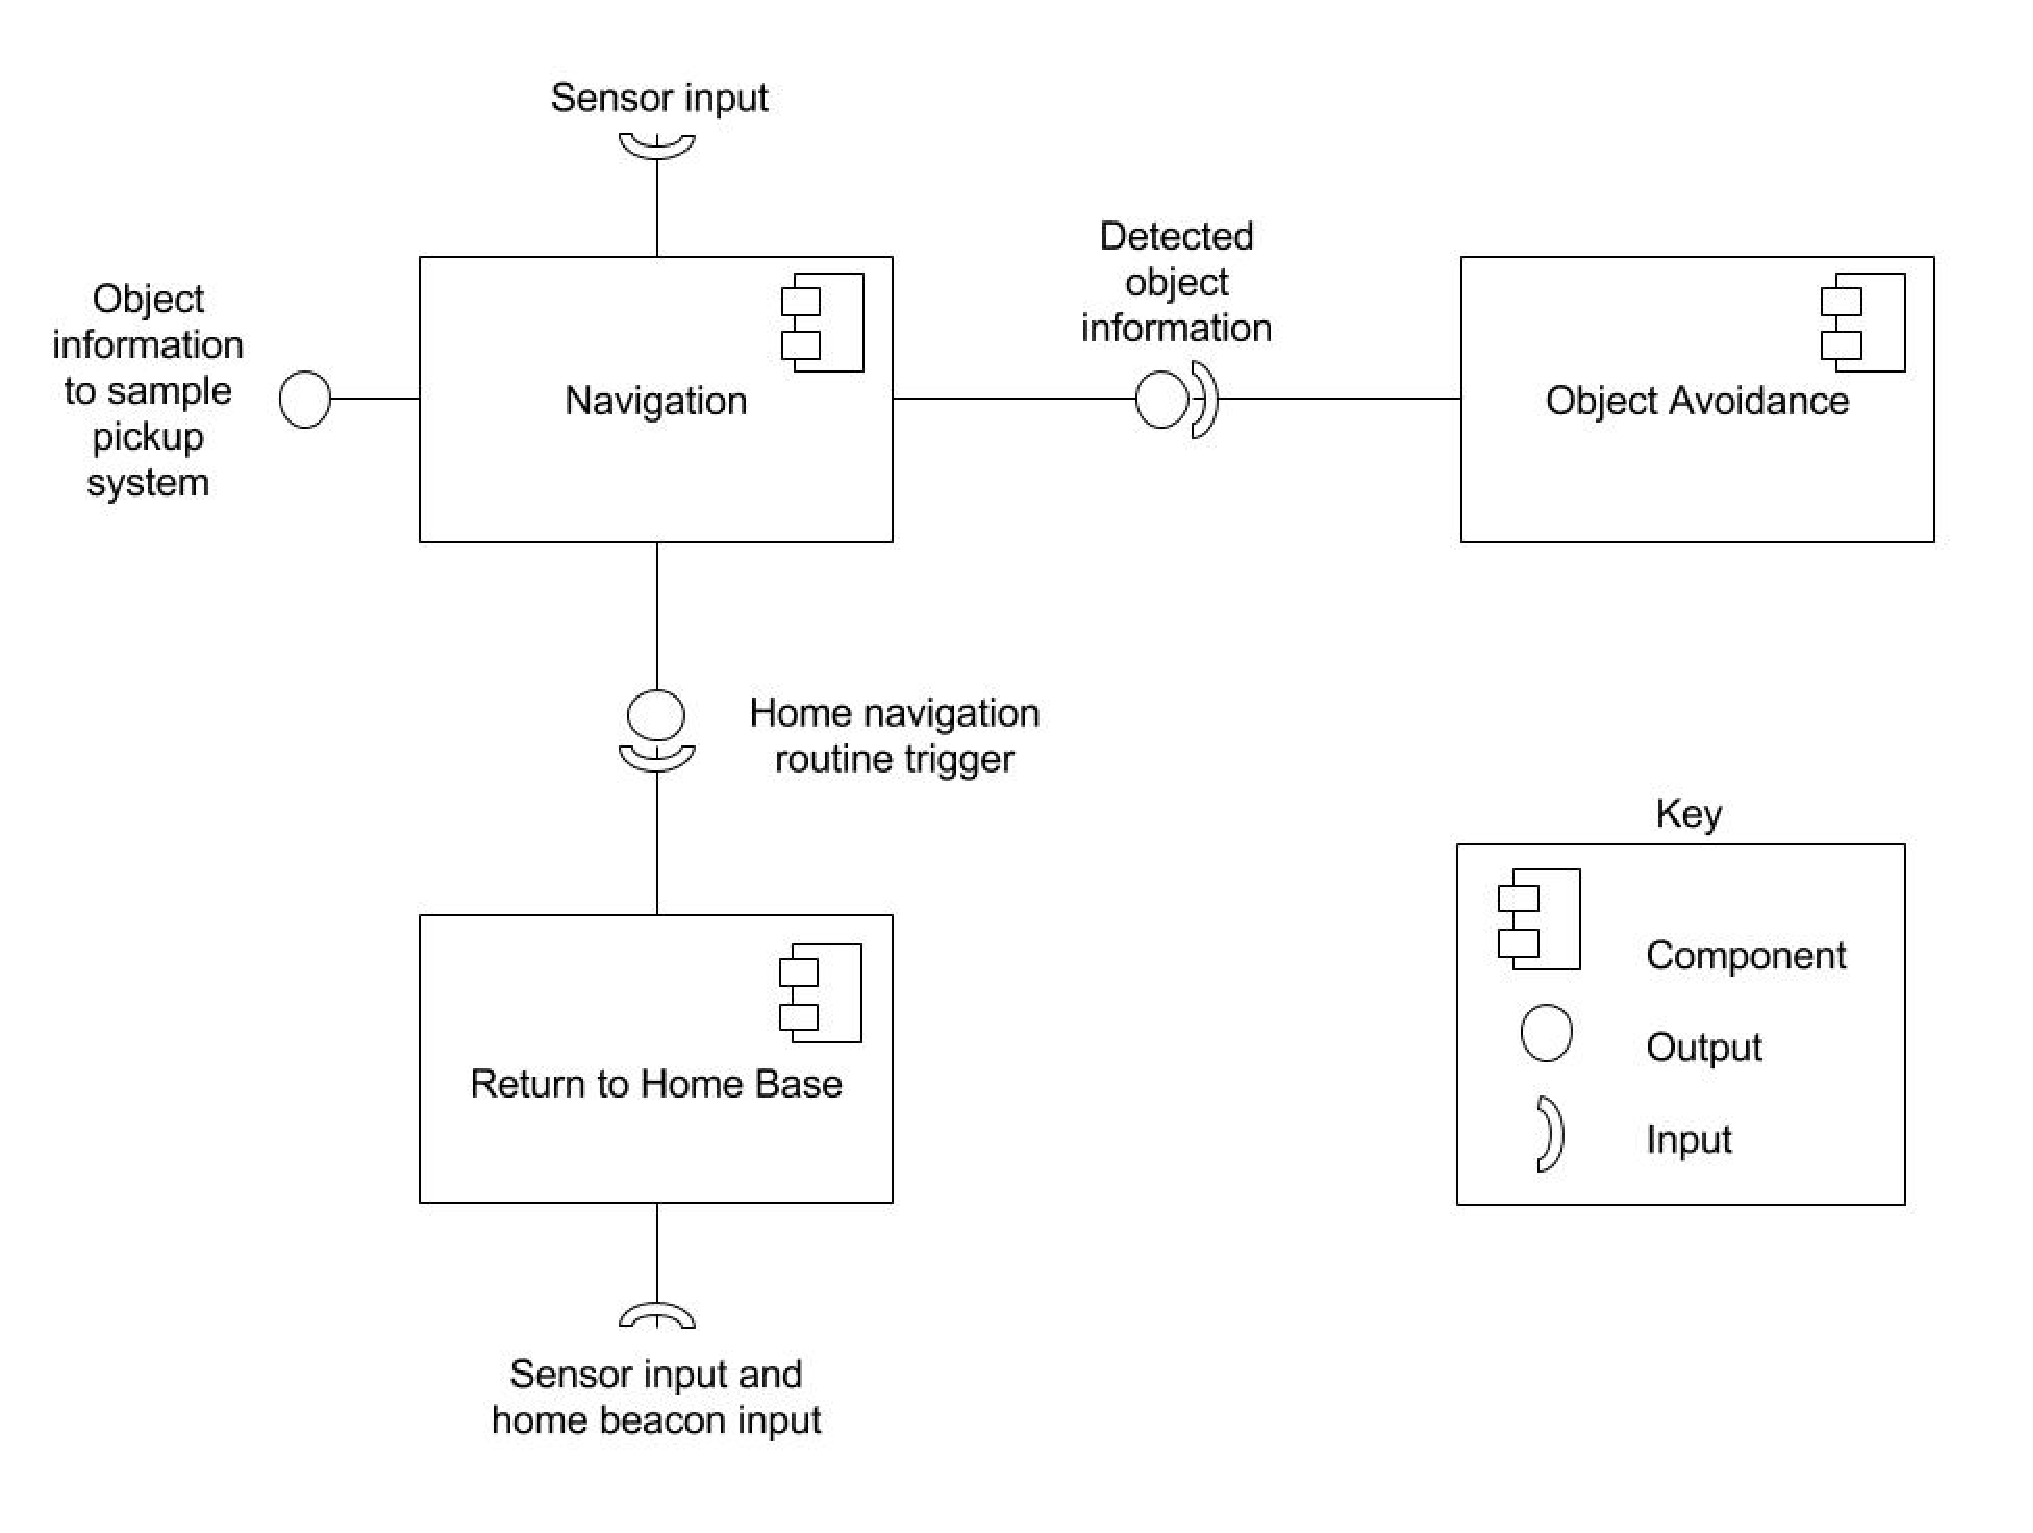
\includegraphics[width=160mm]{drawing.eps}
\caption{UML Component Diagram}
\end{figure}

\subsubsection{Interaction Viewpoint}

The interaction viewpoint addresses the communication of the navigation system with other systems. Component communication is critical due to the rover team approach at development. The electrical and software teams communicate with each other but may not always be able to collaborate when writing code. Views addressing the software design interaction should have well defined communications formats. 

\begin{itemize}

\item View: Operating System

The Robot Operating System has been chosen to address concerns of subsystem communication. ROS is an operating system for robots that implements a publisher/subscriber framework for software node communication. The framework encourages building a system of nodes that communicate, which will work well with our modular design plan. The messaging system makes use of .msg files that follow a distinct form with identification headers, given flexibility on storing communicated messages to be acted on at a later time. This predetermined messaging format alleviates the communication concerns the electrical and sample recognition subteams may have.
\end{itemize}

\subsubsection{State Dynamics Viewpoint}

The state dynamics viewpoint looks at possible states of the design. Determining states of operation helps the other subteams understand the process that a reactive system is taking. Design concerns addressed are modes, states, transitions, and constraints in time ordered events, which are all part of a dynamic system. 

\begin{itemize}
\item View: Three States of Operation

The design consists three states of operation, each corresponding to a module. Additional states will exist within the rover software developed by the other subteam members. The state layout includes state transitions and accounts for interrupts from the sample recognition states. Diagrams are included illustrating planned states which will allow for the object recognition team to determine when their modules may interact with ours. 

\subitem The Navigation State:

The possible navigation states correspond to the navigation modules outlined in section 4.1.1. The navigation process will consist of directing the rover towards a predetermined sample region and analyze sensor input to determine locate objects in the immediate area. Depending on the analysis result the rover may transition to either the avoidance or return home states. The navigation state may be interrupted by the sample collection module. When a potential sample is identified navigation will cease and the state will change to a sample pickup state. 

\subitem The Object Avoidance State: The object avoidance state will be trigger by the navigation state. Using the sensor input the relative distance of the object in question will be determined. A new direction of travel will be taken, with a set distance based upon the object's location. Once the distance has been traversed, the rover will decide the object has been avoided successfully, then transition to the navigation state.

\subitem Return to Base State: The return to base state will be triggered from either a sample recognition state flagging the rover saying that collection is complete, or from a timer on the rover which will elapse when the competition is near its end. The state will determine new a route towards the home base and transition back to the navigation state. 

\end{itemize}

\subsubsection{Resource Viewpoint}

The resource viewpoint addresses concerns about sharing the onboard computer, processing power, and battery power. The outlined design must share resources will other onboard systems so the efficiency of each sub teams implemented systems are critical.

\begin{itemize}

\item View: Resource Sharing

The design of the rover requires that its onboard resources are shared between multiple systems. The key resources which are shared are the processor and the battery. To minimize resource consumption, the navigation system has been designed with minimal components. One sensor system will be used minimizing both processor and battery power consumption.

\subitem Processing Power Utilization: The processor must be shared with other software on the system, including the object recognition software and the robotic arm software. The processor will be a multicore intel processor in the i3 to i7 range. This will afford the rover decent multitasking capabilities, but processing must still be kept to a minimum due to the computationally heavy tasks of the rover. The navigation system itself must process two video feeds to generate depth data which will then be processed further to identify obstacles. To minimize processor use the navigation system will use only one sensor system, rather than a combination of sensors. A low refresh rate will be used by the camera for calculations, as the rover must move under 2km per second so a  high refresh rate is not critical. This will free up processing time without hindering the effectiveness of the navigation and obstacle avoidance system.

\subitem Battery Power Utilization: The rover uses a battery to provide power for the onboard systems so the power consumption of our design is a big concern. Unlike processor utilization, if the battery charge is used up, the rover will cease to operate. Fortunately the methods used to reduce processing power will also reduce power consumption. Reducing the sensor systems to just one greatly decreases power usage. As it is not known exactly how much power the entire rover system will use, the electrical team can now factor in our estimates to help them address the battery concern. 

\end{itemize}

STILL NEED: a discussion of what had to change over the course the year.

\section{Technology Review}

	The team will develop the autonomous navigation system for the Oregon State University Mars Rover. The rover will be competing in The Sample Return Robot Challenge, a university robotics competition hosted by NASA. The software developed will allow the rover to efficiently navigate unknown terrain by using sensor input to avoid obstacles and recognize a base station which it will be able to maneuver back to. The navigation system will integrate with other software systems present on the rover. 

\subsection{Operating system}

	The operating system is the essential base component from which all other software for the robot will be run. This is very important piece of the project because the rover will need multiple sensor running simultaneously in order to complete it tasks. The rover needs an operating system that can efficiently manage the sensor input. Multiple languages will be used for different components of the system which will need to interact with each other at some points. A operating system that is robust, portable, and efficient is necessary for this challenge.

\subsubsection{Robot Operating System}

Robot Operating System, or ROS, is a software framework intended to simplify the development of robotics software. The operating system is intended for collaborative development and uses a modular model to combine code. The creators of ROS describe the software at the lowest level as an interprocess communication system. ROS provides built in libraries and tools to aid in development. The libraries available include localization, mapping, and navigation, all of which may be useful in developing our system. The tools that ROS provides are intended to simplify the development process. Tools include debugging and system state visualization, and rviz. Rviz is a visualization tool that aims to let developers see exactly what their robot sees. Using the communication messages, rviz can build models demonstrating what information the sensors in the robot are gathering, which can be very handy when testing the systems. 
 
\subsubsection{VxWorks}

	A different operating system is Vxworks. It is a real-time operating system (RTOS) developed as proprietary software by Wind River. VxWorks powers billions of intelligent devices, and delivers an industry-leading combination of scalability, safety, security, and virtualization capabilities to meet next-generation requirements. VxWorks is used in industries like aerospace and defense, and in medical devices, industrial equipment, robotics, and consumer electronics. This RTOS can be use in multicore asymmetric multiprocessing (AMP), symmetric multiprocessing (SMP), and mixed modes and multi OS designs on 32 and 64 bit processors. Vxworks is used in some NASA rovers and other projects. A major downside to using Vxworks as our operating system is that it could require a more processing and power than we will have access too. ROS seems like a better option because it is specified for robotics unlike Vxworks which has a variety of usages that we simply do not have a need for.

\subsubsection{Robotic Library}

	Rather than a non standard operating system, another way to program the rover would be to use a robotics library. The Robotics Library (RL) is a C++ library for robot development. This API includes tools to implement ?mathematics, kinematics and dynamics, hardware abstraction, motion planning, collision detection, and visualization?. This would be very useful because testing for collisions will be key in our development in both navigation software and object avoidance. Cameras like the kinect can be utilized with the Robotic Library as well. A negative is that the hardware we are provided with might not be advanced enough to be able to implement this. We also must consider that although we may be comfortable working in C++, the other non software subteams may be writing short pieces of code for their components. Using this library would restrict the team to a single language for the core robotics functions. 

\subsubsection{Conclusion}

	We will to use ROS because it gives us the freedom to work with different languages and collaborate with team members easily. The built in will libraries and modularized design of ROS will help the rover team develop the system efficiently because we will not have focus heavily on interprocess communication. ROS does not restrict our languages options like a specific library might, and because ROS has been used by the club in the past, members of the other subteams will already be familiar with the software which would not be the case if an operating system like Vxworks was chosen. 

\subsection{Depth Sensors and Cameras}

	A critical component of an autonomous navigation and avoidance system is the sensors which collect information about the vehicle's surroundings. Depth sensing technology is required to avoid collisions with obstacles, allowing the rover to navigate to its objectives and search for samples. The team must consider the range of the sensors, processing power to analyze sensor data, and power required to operate.

\subsubsection{Stereo Vision}

Stereo vision is a camera setup which utilizes two cameras spaced slightly apart to gage depth by calculating the relative difference in position for objects in the two different images. This concept is similar stereoscopic vision which most animals use to perceive depth via visible light. When an object is close to the observer, the item appears more to the left in the right image, and more to the right in the left image. As the object moves away, the the ?gap? between the the object in the two images when overlaid shrinks, until there is no gap and the object appears as one uniform image when the two images are overlaid. 
To implement stereo vision, two identical cameras will be necessary and the OpenCV library will be used. Identical cameras are needed to insure that the left and right images are as similar as possible to better calculate the differences in the images which indicate depth. The higher the resolution of the cameras, the more information about the environment will be gathered, and the further that objects will be able to be detected. However, higher resolution image processing utilizes more processing power. 
Another downside is that stereo vision is limited in range. The three factors determine range are resolution, field of view, and distance between the cameras. With stereo vision, once an object appears in the same position in both the left and right images, depth cannot be determined without knowing the scale of the object. Anything past this point of convergence essentially becomes a 2D plane at the point of convergence. If you were to take a 360 degree scan of an environment and create a 3D visualization, you?d get a 3D environment with a dome at the point of convergence which provides a 2D picture of everything further away.To increase the distance for the point of convergence, you can move the cameras further apart, but this has it?s limits, and increases the mimimum distance of depth detection. 
OpenCV is a BSD licensed open source computer vision and machine learning library. The library provides a common infrastructure to enhance the speed, versatility, and ease of development for computer vision applications, making it simple to utilize data from almost any camera or vision system. 

\subsubsection{Lidar}

Lidar is a sensor technology which utilizes reflected light to measure distance. It consists of a laser emitter, and photodetector, and a scanner with optics. To determine depth, laser pulses are sent out, and the distance is calculated from the time-of-travel of the light pulse. This is essentially how a laser range finder functions. To scan an area with LIDAR, the laser is rotated horizontally and vertically to calculate the distance of many points in its target area. Combining the angular and positional data of the range finder with the corresponding distance for each point provides a 3D mapping of the points. Combined this gives a 3D representation of the area that the LIDAR scanned with its laser. 
LIDAR can be a highly effective system for creating a 3D scan of an area, however the LIDAR system available to the OSU Robotics Team has its limitations. For one, LIDAR systems in general do not detect color. Color is not necessary for navigation, but could have its uses in object recognition. More importantly, the LIDAR system available to the team presents its data in an inconvenient form. It does scan a 3D area with approximately a 15 degree vertical FOV and a wide horizontal FOV, however it compresses the data into a 2D horizontal plane. This will show the depth of objects within that 15 degree vertical FOV, but will not tell us any vertical information about the object. For example, if an object was detected spanning the bottom 2 vertical degrees and 5 horizontal degrees in the center of the LIDAR view, data would indicate that there is an object 5 degrees wide directly ahead and would give its depth, but not indicate how high or low the object reaches. The software could not easily determine whether the object was a rock resting on the ground or a tree branch suspended above the sensor. This will make it difficult to figure out whether the rover can go over or under the obstacles and it tough to differentiate between a slope in terrain and a wall. Due to these limitations, the LIDAR system available to the team would not be effective as a single sensor to be used for navigation and avoidance. 

\subsubsection{Infrared Depth Sensing with Camera}

With the recent trend of motion controlled interactivity, new sensor systems have been developed for depth and motion tracking. One popular system is the combination of an infrared emitter, an infrared camera, and a RGB camera. The Xbox Kinect is one of the pioneering examples of this technology. Utilizing the IR emitter and camera, the device can calculate the depth of objects within the IR camera's field of view. The emitter shines a constant pattern of IR dots to cover everything in the IR camera?s view, then the depth of the points are determined by comparing the expected and actual positions of the dots, due to the offset of the sensor from the emitter. This information is then combined with the RGB camera to provide depth information for each of the color pixels, providing a 3D color image. Additionally, devices such as the kinect have an onboard processor which handles the depth calculations, reducing the amount of processing power required by the rover?s main control processor.
The main drawback of this infrared depth and RGB camera system is that the range is quite limited. Most affordable systems, such as the Kinect, have an effective range of about four meters. Further than that distance, they cannot accurately gage depth from the IR dots. These systems are highly effective at efficiently creating an accurate 3D representation of their surroundings, but limited range is a problem for our application. A Kinect like system could help navigate the rover to avoid obstacles short range obstacles, making it quite useful if combined with a system that scans further objects. 

\subsubsection{Conclusion}
 	Currently we are testing to see what combination of sensors will work best together for the navigation and avoidance team. We have yet to come to a clear decision but have a plan. Since we are not limited to just using one set of sensors, stereo cameras will likely be mounted on the front of the rover. We have many models to chose from. These will analyze the objects in front of the rover and determine if obstacle avoidance is necessary. A LIDAR unit will likely be mounted on the rover as well. The LIDAR will be a component for our choice of navigation algorithms.

\subsection{Mapping and Navigation Strategies} 

Competition rules bar using earth based sensors on the rover, meaning something akin to GPS cannot be used to help the rover know where it is on the course. The competition is timed, so the rover must not search areas multiple times or maneuver efficiently. To ensure the rover can navigate efficiently, an algorithm that utilizes sensor input to map the environment or provide navigation instructions to the rover is desirable. 

\subsubsection{Simultaneous Mapping and Localization}

	Simultaneous mapping and localization, or SLAM, is a set of algorithms which are used to create a map of an environment while also using that map for navigation purposes. Although the algorithms can work with varied input, the mapping libraries included in ROS require that the robot in question implements an odometry technique and a laser range finder. Odometry allows the robot to use sensor input to determine distance moved. In the context of the mars rover, this may be generated by wheel rotation. The rotation must be measured accurately for SLAM algorithms to work well. For general applications of SLAM algorithms the range finder does not need to be a laser, however the ROS mapping library specifies that a ?horizontally-mounted, fixed, laser rangefinder? is required. The lidar system that the robotics club has meets these requirements. 
The mapping algorithm is based on changes in odometry. Using the rangefinder input, a map is generated which includes the surrounding environment. As the robot moves along a path, changes in odometry trigger updates from the range finder. The new input from the rangefinder is analysed and compared with the map generated by the older analyses to determine the robot's location. Information which does not correspond to something in the current map is then added to it. Using a combination of odometry and range finding, the robot more accurately know where it is than if it was just to rely on one or the other. 

\subsubsection{Dead Reckoning}

	Dead reckoning, or DR, is a navigation process which bases navigation on the known starting location of the robot. The idea behind dead reckoning is to estimate the robot's current position based on a starting point, and utilizing movement speed with a direction and time traveled. Due to the nature of estimating position of a starting location and travel time, DR is very susceptible to cumulative errors. If the speed of travel or direction is not measured accurately, future calculations will become less and less accurate.
	With a dead reckoning procedure object avoidance becomes another means for error. Rather than traveling in a constant direction or along an anticipated route, the algorithm must be interrupted with an avoidance routine. When avoiding an obstacle the robot will most likely need to deviate from the current path, navigate around, and return back to the path it was previously on. As the direction of travel is changed during avoidance, the likelihood of errors being introduced increases. 

\subsubsection{Pilotage}

	Pilotage is a navigation process that utilizes a fixed visual reference on the ground and sight or radar to find its destination. Pilotage navigation can be used used for guiding vessels, aircraft, hiking and scuba diving. Due to the competition rules, the rover would need to utilize a camera or lidar for sight, since radar is not allowed. Pilotage is best used when close to the land or reference points are available on land. Without references to help navigate, another navigation strategy, such as dead reckoning is needed. In our application, a down side to pilotage is that the sensors will need to be able to recognize visual references to function best. With poor visibility due to the terrain of the course, another strategy will need to take over for navigation. This means two navigation systems will need to be developed and tested rather than one. The map provided to teams in early January however, could make pilotage a viable option depending on the level of detail provided. If we have enough information about the landscape then a set of points of reference could be chosen. 

\subsubsection{Conclusion}

	The team will be using simultaneous mapping and localization algorithms as the primary navigational tool for the rover. This technology was selected because with ROS has built in SLAM libraries for use with lidar. Using a navigation method that is packaged with ROS ensures we have the debugging and simulation features that ROS provides at our disposal for development.

\subsection{Base Station Beacon}

	The competition requires that the rover be placed on a base station to begin the challenge. The station is an elevated platform with ramps on the sides, with one side extended  where each team is allowed to place a home beacon. The beacon is constrained by the same technology rules as the rover, which includes no earth based sensors. The beacon must have footprint of no more than 2.0 x 0.43 meters and can not be taller than 2.0 meters at the beginning of the competition. 

\subsubsection{Checkerboard Image}

	In previous years the mars rover club used an image as the beacon. A large black and white checkerboard image was placed vertically behind the base station for the rover to look for when it was ready to return to the home base. The team found this to be a viable solution, and estimated that the rover could locate the image well at a distance of about 30 meters. To best recognize the image the rover needed to be at an appropriate angle, making the direction of travel towards the home base important. Using a vertical image as a beacon behind the rover also constrains the starting direction the rover may travel in when it begins on the course.

\subsubsection{Radio Localization}

	Radio localization is another viable beacon implementation. Using radio localization has been discussed by the team in the past but has not come to fruition. This year the electrical team is prioritizing developing a radio localization system that will allow the rover to calculate its distance from the base station. Once this project is completed, the team will improve the radio system to allow for the calculation of angle from the base station too. Advantages of radio localization include that it will does not depend on the direction of the rover and the base to function and have a long range. Depending on if the electrical team is able to get the full radio system working, knowing the angle from the home base could be advantageous when driving back towards the home base. Depending on the height of the radio system, the rover may also be able to travel off the back of the station at the start of the competition. 

\subsubsection{Infrared Beacon}

	Infrared technology could also be used for the home beacon. An infrared light emitter on the base station would function similarly to the radio beacon. The infrared beacon would allow the rover to calculate distance to the base station. The receiver could be mounted in a specific position on the rover and the direction of the home base could be obtained in relation to the rover. An IR beacon would be susceptible to interference. Obstacles in the course or a change in terrain height could obscure the beacon and interfere with detection. 

\subsubsection{Conclusion}

	The home beacon will use localization technology. At this point in the rover team developement, radio localization is not ready, although it is ideal for the application and the most efficient localization method of the technologies reviewed. Radio localization is preferred because it is not as susceptible to interference from objects between the rover and home base. The infrared technology is available to us now and will be our backup if the radio is not developed in time by the electrical team. 

STILL NEED: Did you change your mind about any technologies?

\section{Blog Posts}

Your team weekly blog posts. These should be formatted nicely and clearly distinct from one another.

\subsection{Welcome to my blog!}
by Riemer, Ian James at 11:51 AM
This is where I'll be sharing my thoughts on topics that matter to me. Who knows... I might even share pictures, videos and links to other interesting stuff.

If I catch your interest, let me hear from you.


\subsection{General updates after TA meeting}
by Fenton, Jay Louis at 5:01 PM

General updates after first TA meeting:

Meeting schedule:
\begin{itemize}
\item Mars Rover Team, Sunday 2pm
\item TA Updates, Monday 2pm
\item Rover Software Subteam, Monday 6pm
\item Project Advisor Updates, Friday 12pm
\item Team Meetings, weekly, when schedules align best
\item OSU Robotics club, no set times yet
\end{itemize}

Mars Rover Team meetings:

10/18/15 - General mars rover discussion. Each subteams role was discussed and it was noted leads were still needed for both mechanical and software.
10/25/15 - Discussion of past strategies and problems run into in the past two years of competition, as well as a discussion of rule changes. Chosen subteam leads introduced to the club. The challenge has been confirmed to be taking place this year.

TA Updates:
10/26/15 - Met with TA and learned his role and what to expect in our weekly meetings.

Rover Software Subteam Meetings
10/26/15 - First meeting tonight
Project Advisor Updates: 

10/7/15 - Introduction to the project and discussion of the Sample Return Challenge. Went over our projects and goals to help determine what to put in our abstracts as well as first task: Install ROS stable version (Indigo) on a Linux machine.
 10/16/15 - Discussed the challenge in more depth and were asked to begin playing around with ROS tutorials. We will get cameras soon to work with as well. Went over our problem statement.
10/23/15 - Discussion of changes to the rules this year. Phase one is now split from phase two, and we are required to submit a video showing we are capable of completing phase one a month before it takes place. The first phase requires us to not only pick up the pre-cached sample as we expected, but also collect one easy sample. Brainstormed new ideas for the home beacon, maybe using IR, but radio localization also a good option that the club has wanted to implement in past years. New assignment: read through the updated 2016 competition rules and keep playing around with ROS. Also talked about what was expected for the requirements document.
Team Meetings:

10/07/15 - Meeting to write the abstract after our first meeting with the advisor.
10/13/15 - Meeting to write the problem statement
10/16/15 - Meeting to create the Sharepoint website and blog
10/23/16 - Meeting to outline requirements document.
OSU Robotics Club Meetings:

10/8/15 - First club get together, turned out to be more of an introduction for students who were interesting in joining.
10/15/15 - General club overview with presentations from each team lead as well as club officers. 

\subsection{Weekly update}
by Fenton, Jay Louis at 4:19 PM

This Monday (10/26) we had our first rover software subteam meeting. This was more of an introduction to the project for those who are not part of either senior design group. After the meeting the link to the rover Github was sent out so we have no had a chance to start checking out how automation and navigation has been approached in the past.

We also met as a team on 10/26 and 10/28 to draft and finalize our requirements document/gantt chart. 

Today (10/30) we had our project team meeting with Billy. We talked about some current ideas for approaching both navigation and avoidance as well as object recognition. Each team received a camera to begin playing with. Given what we know about previous year approaches and the course size, it seems a Xbox Kinect (which we have access to) may be a viable vision option. Knowing depth is helpful for object avoidance and Ian thinks this may be a good approach. 

This weekend we will continue to work with ROS and play with the new camera. 

\subsection{Addtional task and update}
by Fenton, Jay Louis at 8:45 AM

Not mentioned in the previous weekly update was the task of creating a new block diagram. Billy asked us to develop a block diagram for the Req Doc assignment, and has given suggestions on how to improve it. The new diagram will outline the states our navigation system will cycle between. Such as navigating to sample area/searching in area/object detected/object determined to be obstacle, etc.

We also had the general team meeting yesterday and the electrical team thinks that the lidar we have to use is promising as a component we can add to the rover.

\subsection{Weekly Update}
by Fenton, Jay Louis at 2:14 AM

Monday Nov 2nd: The evening software subteam meeting covered camera technology and the two "sides" of the project, navigation and avoidance or object recognition and sample collection. 

Wednesday Nov 4th: The object recognition team created their state block diagrams and sent them to us. They included sections where there code would interrupt our navigation to take control of the rover, and also created an broader state diagram relating the two teams software. 

Thursday Nov 5th: The team met to rework our block diagrams as requested by Billy. The block diagrams now focus on states of the rover's navigation system and transitions to the avoidance and return home phases. These are similar to the diagrams created by the object recognition team.

Friday Nov 6th: Subteam meeting covered previous camera placement on the rover and current camera options. Both teams will do an analysis of the camera options in the following week and determine which cameras seem most useful. Criteria used to select cameras will be power use, sensor requirements, ease of processing sensor output, color detection, and compatibility with system. We will also work more on our revised design document and the technology review. 

\subsection{Weekly Update}
by Fenton, Jay Louis at 9:36 PM

Sunday Nov 8th: The weekly rover team meeting covered strategy and together we ranked the camera/system requirements in terms of navigation. We used a series of criteria and voted which were most important. Example criteria we accuracy, efficiency, ability to recover from error, etc. 

Monday Nov 9th: The team had the weekly TA meeting and discussed the changes that should be made with the requirements document. The team implemented the changes to the requirements doc after the meeting and resubmitted it via Sharepoint.

Tuesday Nov 10th: The team met and worked on the tech review.

Wednesday Nov 11th: The team worked on the final draft of the tech review in the morning and submitted it via Sharepoint.

Friday Nov 13th: Both software subteams had the weekly meeting with Billy. We discussed the tech documents and our approach to selecting cameras. Although lidar with SLAM is promising in terms of ease of implementation with ROS libraries, it is worth noting that the level one cause is not the same as level two this year. Since SLAM algorithms rely on objects for reference and some team members suspect the course will be a football field, SLAM may not be efficient. Lidar can also be used for localization with some ROS libraries, so we will research those too. Ian suggested using Optical Flow to get a bearing on where the rover is. The team though this was a very promising idea. 

\subsection{Weekly Update}
by Arreguin, Alexander at 3:22 AM

On Sunday Nov 15: The general meeting happened once again at 2pm. 

Monday Nov  16:  We discussed the technical review and talked about the Preliminary Design Document with oscar. He made it clear how technical and descriptive we need to be with the assignment to accomplish our goal.

Tuesday Nov 17: The team met once again and finished the technical review. We revised everything thoroughly to make sure we correctly completed the assignment. 

Friday Nov 20: The senior team met and discussed what we need completed by this term and what we will be starting next term. The general idea is to choose the cameras we will be utilizing by end of fall term. Next term we will be focusing on implementing the rover so we can successfully have it working for the competition.

\subsection{Weekly Update}
by Arreguin, Alexander at 5:39 PM

November 30 - Had our weekly advisor meeting discussed our progress throughout the term and what we are planning on doing the next 9 months. Also talked about the design document and what was expected from us on it. 

December 1- Practiced speech for class. Had to give a 30 second speech about our project to our class. It was a success as Jay, Ian and myself spoke evenly about our project. 
Worked on the design document. Very confusing design we needed to follow for this assignment. 

December 3- Worked on the design document. The weekly software team meeting was cancelled this week. 

December 4- Met with Billy and the rest of the senior software team to discuss plans. We have to decide what cameras we will utilize by the end of next week. A specific timeline has been made for next term with dates. See Below.

Navigation Team
\begin{itemize}
\item 1/1 - Get camera input (shared)
\item 1/15 - Make decision on how to use map data
\item 2/1 - Recognize obstacles
\item 2/16 - Complete decision strategy on obstacle avoidance
\item 3/1 - Complete home base strategy
\item 3/1 - Communicate information with Object Recognition Team (shared)
\item 3/18 - Have initial code completed for State machines
\end{itemize}

\subsection{Week 1 Update}
by Fenton, Jay Louis at 7:27 PM

Over the break a new stereo camera was purchased. The two capstone teams will share this initially and decide if another should be purchased in the future. Two webcams were also purchased. 

Friday 01/08 we met with Matt, a graduate student familiar with robotics. We discussed the two phases of the challenge and his ideas of how we might approach them. He agreed with our dead reckoning method for level one, given that there will be no obstacles on the course so slam would be ineffective. 

For level two he suggested a 3D slam algorithm. Since the team will receive a topographic map of the field, he though that this may be able to be fed into the slam algorithm as an initial condition and allow the slam generated map to already have information prior to the competition. We also discussed the issues of tracking the rover via odometry or slam especially with hills. Matt will be a good resource we can discuss plans and challenges with, and he offered to introduce us to another graduate student who may be able to help with 3D slam.

We had our first all team meeting on 01/10 and discussed the plans for this term. The electrical team made progress on the rovers uniboard this break, and the mechanical team is hoping to wrap up their projects by February. We took a look at the maps that are out for us to use along with the new competition information. The level one map is as we expected, a portion of a football field with no obstacles. The object regions are very small and a square route around the field should suffice. If the odometry works well enough on the rover we should be able to navigate this phase with minimal reliance on any cameras which would be ideal.

The level two maps are also as expected, and the object regions smaller than we anticipated. Interestingly, 15 regions are shown but we expect only 10 objects to be present, so 5 may be false areas. The map also provides landmarks, which may be something else we can seed our slam algorithms with!

The first subteam meeting will take place tomorrow evening.

\subsection{Additional Week 1 Note}
by Fenton, Jay Louis at 7:45 PM

We had our first TA meeting of the term and discussed what was expected of us this term. We have a video presentation and progress report that will be due when the alpha is submitted at the end of week 6. 

\subsection{Week 2 Update}
by Fenton, Jay Louis at 1:24 PM

This week we got our new webcams up and running, and also got still images from the new stereo camera. The cameras were a little tricky to get running due to most team members running VMs, but once we determined the issue they could be used plug and play, as we expected. The still images were due to the fact that the camera requires an Nvidia graphics card, which none of us had in our laptops. Our new computer has one, and that computer arrived late this week. We got it up and running Sunday afternoon, installing Ubuntu 14 as well as ROS Indigo. We tested the new cameras with it. 

We met with our TA and will revise our requirements document before the next meeting to ensure they requirements make sense for the competition and our task now that we have more information and have new equipment at our disposal. 


Our current weekly work schedule is as follows:

Sundays post rover team meetings for ~4 hours.
Monday during and after software subteam meetings for ~2 hours.
Tuesday and Thursday evenings for ~2 hours each night. 

\subsection{Week 3 Update}
by Fenton, Jay Louis at 8:10 PM

This week the team met at our usual times, Mon, Tue, Thur, evenings as well as Sunday. Our midweek meetings covered some new open CV code and ROS camera drivers. We are able to use the drivers from the 2014 rover as well as newer ROS drivers if desired. Once the drivers are running we subscribe to the specific topics they publish with nodes that we write. This should mean the open CV code we've written can be drag and dropped into a subscriber that uses the open CV Bridge. This is also where our octomap nodes will come into play, subscribing to a point cloud topic that our stereo camera drivers publish. We can have nodes for the object recognition team subscribing to the disparity map that is published, allowing us to use the stereo camera for two very different applications. 

Our goals for this week include getting octomap running as a node subscribing to topics published by our camera drivers in ROS, and evaluating the webcams vs stereo cameras in terms of visualization effectiveness and power consumption.

\subsection{Week 4 Update}
by Fenton, Jay Louis at 11:28 PM 

A little late but some good progress has been made. I got the computer back from Chris who had had some issues with it and needed to reinstall Ubuntu. I got ROS, opencv, and the ZED SDK downloaded as well as the nvidia cuda toolkit, a requirement for the sdk. Compiling the ZED camera drivers failed due to a toolkit issue which I have not yet resolved. I have the computer at my house and will hopefully have it working tomorrow morning (Feb 11). Then with successful compilation we can move on to getting the octomap sever node I have on my computer subscribing to a point cloud generated from the stereo camera, and get some better visualization going. 

\subsection{Week 5 Update}
by Fenton, Jay Louis at 12:27 AM

This week all the week 4 issues noted were resolved. Once the ZED provided drivers were running, the topics in ROS were familiar and easy to work with. The stereo proc node which I was attempting to use as a driver before was actually intended process topics provided by another driver. This node provides us with a variety of processed stereo camera topics. Of particular interest to the project is the point cloud 2 type topic. This can be mapped to the input of an octomap server. By remapping topics that the octomap server generates, we can use RVIZ, a ROS visualization tool, to view our generated 3d occupancy maps. We have the ability to alter the distance that the octomap "builds" at, but this building area is limited by the point cloud itself. The point clouds have been tested heavily indoors and seem to have a larger range than needed. With octomaps generating 7.5 meters from the ZED camera we see good mapping results and the point clouds extend further. 

We began the write up for our alpha and have the video to work on this week. We also need to tackle our timeframe challenge, which is a needed input to generate octomaps which build and improve as the camera moves. Since we are testing with only a camera and no other sensors, the octomap is seeded with a static transform. This is still an area we are researching and functionality for the alpha does not depend on it. 

\subsection{Week 6 and 7 Updates}
by Fenton, Jay Louis at 10:23 PM

The week 6 update comes a little late, we spent the week making sure the alpha was ready, writing our paper and creating the video presentation. The final work done for the alpha was to connect the navigation node to the octomap server via another subscription. 

Week 7 was focused on working with ROS transforms, which allow different sensors to translate data from their coordinate frames of reference to other frames on the robot. We will have transforms between the base\_link, our rover, the camera\_link, the ZED stereocamera, and another link for the odometry. Right now the rover is build and includes two wheel encoders. This will be the odemtry we work with first but other sensors may be added in the future. We had some trouble with the transforms between the rover and the camera since we need to determine what data we want transformed, and create a transform specific to that type or find one already available. As of now the plan is to translate the point cloud 2 data that is already processed using the pc2 library. Functions exist to do this but have some unclear arguments. 

Once the initial transform is created we then hope to start working with the rover and controlling it. From there we can try to set up another transform with the encoders.  

\subsection{Week 8 Update}
by Fenton, Jay Louis at 6:00 PM

Been working with the transforms a bit more, had luck getting the include issues worked out. Everything is compiling now locally, but it still needs to be tested on the rover computer. 

Ian has been looking more into working with the topographic map and has found a process to convert map information to an oct tree form. 

For the beta we would like to get the rover moving. This means getting another transform for the odometry connected with the octomap server as well as getting the nav code running. We will need to work with the other subgroups to do this since it will involve mounting the computer on the rover and adding code that interfaces with the hardware which we have not done yet. The other teams have been more focused on the arm since their is a discussing about creating a new arm entirely if the current arm is determined to not be suitable. 

\subsection{Week 9 Update}
by Fenton, Jay Louis at 4:10 PM

The TF compilation issues were resolved, and after some work running properly as a service broadcaster and listener in ROS form. ZED also released new drivers last week which not only produce left and right images, but now produce a pointcloud as well. This PC2 is much more detailed than what we previously have worked with. This means our maps are less noisy and have better defined surfaces present. 

Ian was successful in translating a Google map surface into an octomap compatible file type. This file type be used as a command line argument in our octomap launch file. We still need to work with this more to get it working properly. 

Two software team members got an optical flow sensor working via an Arduino and reported at our weekly meeting. This sounds like a viable option for the odometry on the rover, however it needs to be tested further and compared to other odmetry options, like the wheel encoders. 


\subsection{Week 10 and 11}
by Arreguin, Alexander at 11:14 AM

The rover is finally finished and implementation on it will finally begin start of next term. Met with the robotics club during week 11 (finals week) to plan dates and times to begin testing. We had till April 8 to submit a video of level 1 functunality. The video must traverse 5 meters, collect a competition sample, traverse 5 meters with the sample, return to the starting point with sample and get it all on video. 

\subsection{Spring Break and Week 1}
by Arreguin, Alexander at 11:25 AM

During spring break Alex met with Nick Ames and others to learn about the rover. It was a brief meeting and simply learned how to start the rover and things that still needed to be worked on. 

Week 1 has started and the deadline of April 8th is approaching quickly. We got a week left to finish the video and submit it via youtube. A link will be posted once finished.

Since the wheel encoders aren't ready we are using optical flow for distance measurement. We have also started working on the home beacon recognition. The radio doesn't seem to be ready for us to use, so we are working with the checkerboard to be detected by the rover to return home. 

\subsection{Week 2}
by Arreguin, Alexander at 11:44 AM

We finished the video and submitted it. We actually accomplished this two days before it was due on Wednesday night. We stayed pretty late in the lab working on the rover trying to accomplish our goal.  

\begin{itemize}
\item \href{https://drive.google.com/open?id=1lH9-26Qdjt1_Ppa7h6n0BpqmCCp4h-UH45eNqOTPJ3U}
{Level 1 checklist}

\item \href{https://www.youtube.com/watch?v=H8sDekAOodg}
{ Level 1 functionality}
\end{itemize}

Even though we didn't use the checkerboard recognition for the video, it is now working. More testing still needs to be done with the rover but the distance the zed camera can read the board on a constant find is about 20 to 30 meters. It can also detect weather it is the front of back of the board. The angle it gives us is fairly accurate but more testing needs to be done to determine exactly how accurate it is.

\subsection{Week 3 Update}
by Fenton, Jay Louis at 12:26 AM

This week we got wheel encoder functionality working. A new node was created which publishes reported RPM for the left and right middle motors. 

Data was collected in trial runs using the odometry to aid in tuning the PI controller for distance. Runs were taken at a constant speed for 10 seconds. 4 trials were done, with the optical flow sensor mounted at 4 different heights. encoder values and optical flow readings were recorded from the runs. We also noted the X,Y offsets from the starting location.  

All cameras have been set up to run simultaneously on the main computer, and udev rules created to ensure they will properly launch after a restart of the computer. A udev rule was also created to alter the uniboard permissions on startup. A master launch file was created to handle the camera launches and uniboard communication node. 

Moveit was also locally installed and worked with briefly, this will be a greater focus in upcoming weeks. 

The current team goal is level 1 functionality by this Friday

\subsection{Recent Updates}
by Fenton, Jay Louis at 7:08 PM

We our on our way towards complete level 1 functionality. Ideally this will be completed before the Engineering Expo. Currently we are working with the ROS 2d navigation stack to generate costmaps and plan paths. This stack is designed to work with transforms from stereo cameras (which we already had written) and with a transform from our odometry, which was written last week. 

We can supply a pre built .pgm map to the nav stack to initialize the global boundaries. The local obstacle avoidance is handled by the stereo input. The navigation stack outputs a velocity vector to direct the rover. Since rover is differential drive, this vector only has x velocity, and a z angle. We will subscribe to this velocity vector and then use the velocity PID to control the wheel rotation. 

We fixed the computer startup issue when the stereo camera was plugged in at launch, and wrote a bash script to automate the rover startup when the computer is run. The Zed also had trouble running when the VGA port was empty, and the team has created a device to spoof this so the computer can be placed within the rover. 

\subsection{Week 6 Update}
by Fenton, Jay Louis at 2:10 PM

This week was focused on creating the video for our expo level software release and finalizing the paper. We also worked on odometry testing during the week. We had great results testing the optical flow on the turf, the quality readings displayed by the optical flow node were the highest we had ever seen. Our movement is easily trackable when we are on a linear path. I was able to use pre recorded bag data to simulate the rover moving known distances to goals.

This week we aim to put to get the movement goals with the other capstone teams pickup routines. To deal with rotation we are waiting on the IMU. Our electrical lead has stated he plans to have the IMU accessible to us by this following Sunday. 

\subsection{Week 7 Update}
by Fenton, Jay Louis at 10:27 PM

Odometry testing has gone well. We can rely on the optical flow for all our linear movement and it has now been calibrated. We only have one remaining issue here, and that is with the PID. The PID works very well for getting us to the location dictated from the navigation stack, however it does not work reliably after. There is some bug in the PID that we have not found. If we do not discover the source of this problem we will turn the PID off once our goal is met. 

We have access to the IMU as of today via the uniboard API. This will provide the data for our turning and work with our optical flow. 

The navigation node has been worked on further and now accepts an array of coordinates to send as goals, sets and alters ROS parameters as a means of node communication, and uses a ROS service to communicate with the home base locator node. 

More testing will take place this week concerning the IMU and another goal is to have tests with both teams code working together taking place.

\subsection{Week 8 Update}
by Fenton, Jay Louis at 3:53 PM

This week was focused on preparing for the engineering expo. We wanted to have all portions of the project mostly working so we could discuss them with anyone who asked questions. This meant working on the start up routines, node communication between the two capstone teams, and finalizing our goal order for the level one software. 

We got access to the IMU onboard the rover the day prior to expo. This will be used to provide information about turning. The original plan was to use the encoder differences for this, but one encoder has been reporting bad values which makes our angle estimate very unreliable. The encoders also do not always report valid data since the center wheels stick during slow in place turns. The IMU has been integrated into the odometry topic as well as the velocity PID. 

This week the team is testing the full system. Our startup routines are working but we will need to test them running altogether and ensure there are no errors. Once we are satisfied full level 1 autonomous testing will begin. We will also begin our final paper and create slides for the final video presentation. 

\section{Poster}

Your final poster, scaled and color-printed on a single 8.5"x11" paper. If you don't have access to a color printer, I will print it for you. Let me know.

\section{Project documentation}

STILL NEED:

\section{Project Structure and Development Evironment}
\subsection{The Robot Operating System }
To develop the navigation system the team is using The Robot Operating System, ROS, a software framework intended to simplify the development of robotics software. The operating system was designed to foster collaborative development and uses a modular model to organize code. The creators of ROS describe the software as an interprocess communication system. ROS provides built in libraries and tools to aid in development. The libraries available include localization, mapping, and navigation, all of which have been useful in developing our system. Tools included allow for easier debugging and provide system visualization. Rviz is a visualization tool that aims to let developers see exactly what their robot sees using ROS message types. Message types are data structures ROS provides for communication. They are defined such that nodes written in different languages can still communicate with each other. Rviz allows us to view what our rover would be seeing so we can ensure that the maps created correspond correctly to the environment. Rviz has been a very helpful feature in our map, camera vision, and navigation testing. It is also great for showing the rover team our progress since this is something they are all curious about.

A ROS program is contained inside of a folder, referred to as the ROS workspace. The workspace houses a source (src) folder where the code packages are located. Packages contain nodes that can function in four ways. A node may publish topics, subscribe to topics, broadcast services, and listen to services. Nodes that work with services still work with ROS message types, the distinction is that service communication is a request and reply model as opposed to the publisher and subscriber model. ROS utilizes coordinate frames to manage sensor input. A robot may have many coordinate frames corresponding to moving parts or mounted sensors. ROS transforms are defined to manipulate ROS messages from one coordinate frame to another. Launch files are a ROS filetype designed to make starting programs simple. Launch files are especially useful for starting nodes that the programmers did not create but wish to utilize. The launch file can specify the package to launch as well as topics to subscribe to or publish. 

\subsection{The ROS 2D Navigation Stack}
The ROS 2D Navigation Stack is a collection of nodes which when combined, can provide movement instructions for a robot based on sensor input. We are using the navigation stack to develop our level one software. The core of the stack is a node called \texttt{move\_base} which maintains a local and global costmap of the robot's surroundings. The global map can be seeded with a grayscale PGM file, and the local map updated in real time by a stereo camera. This allows us to use the path planning nodes for goals and use the costmaps as a reference to determine the route that the nav stack outputs. The stack subscribes to similar topic types as the \texttt{octomap\_server} meaning most of the code written for our Octomap testing is still in use.

\subsection{The Octomap Package}
Octomap is a 3D mapping framework based on octrees that will provide the map generation for our level two system. The Octomap library generates a 3D occupancy grid and provides data structures defined as ROS message types. The Octomap creation is managed by an \texttt{octomap\_server} node. The map models arbitrary environments and can be iteratively updated by adding new information from sensor readings at any time. While the distinction between free and occupied space is essential for safe robot navigation, information about unknown areas is important for autonomous exploration. The extent of the map does not have to be known in advance because it is dynamically expanded as needed. 

\subsection{Code Organization}
The team code is contained in a single workspace, divided into a series of packages. Packages include the ZED drivers, transform services, navigation goals, 2D navigation, odometry, wheel encoders, velocity proportional integral derivative (PID) controller, and uniboard communication. The object recognition capstone team's nodes are also present within the workspace. Working code is checked into the robotics club \href{https://github.com/OSURoboticsClub/Rover2016}{Rover2016 Github} repository. 

\section{Level One Theory of Operation}
\subsection{2D Navigation Implementation}
We used the ROS 2D Navigation Stack as opposed to 3D Occupancy maps to achieve level one functionality. Octomap is well suited for obstacle filled terrain and varied ground level, while the ROS navigation stack provides more appropriate tools for navigation on flat ground. Nodes in the navigation stack and the \texttt{octomap\_server} node subscribe to similar topics, utilizing three dimensional point clouds as a sensor input. Point clouds are plots of points that determine the surface of the features in an image. These clouds are generated from stereo images. The navigation stack node \texttt{move\_base} handles the point cloud input and uses minimum and maximum height parameters to isolate potential obstacles. In the case of Octomap, the occupancy map is generated from the point clouds. The maps are maintained by the \texttt{octomap\_server}.

Level one functionality includes generating the coordinate frame transformation tree, which defines transforms between different frames of reference with respect to the the rover footprint, producing filtered odometry topics, running the navigation stack based utilizing the appropriate topics, and sending goals to the navigation stack. The stack outputs a velocity vector which is input into a PID controller that we use to send wheel movement values to the rover. Our level one program node structure is outlined below in the Rover Configuration section. Integration with the sample collection teams code is handled by the ROS parameter server. A boolean parameter controls which nodes run at what times. This is toggled and control is transferred when certain actions, such as successful completion of a navigation goal, have been met. 

\subsection{Launch Files and Startup}
To run the navigation code, we have a series launch files that launch nodes sequentially. Launch files are ROS files that can initialize multiple nodes at once. The launch order is important because some nodes rely on having specific ROS topics available, however some nodes do account for out of order startup and wait for their subscriptions to appear. The previous years code uses a similar launch process, automated in a bash script. We use a bash script that runs launch files on startup of the computer.

\subsection{Rover Configuration}
\begin{enumerate}
\item The ZED Stereolab drivers are launched and produce a number of topics related to the left and right cameras. The diver node is contained within the \texttt{zed-ros-wrapper-master} package. In our alpha level build the ZED drivers did not produce a \texttt{pointcloud2} data type (Figure 1), which is used by the navigation stack. A driver update added this functionality, eliminating a stereo processing node we previously used.

\item The \texttt{base\_move\_param} is set to false in a launch file which denotes that the navigation code is active. When this parameter is toggled to true, the navigation code halts, and collection code takes over. 

\item We launch two of our transforms as a node. Three reference frames are produced by the ZED drivers. The transforms node defines a fourth frame called \texttt{base\_link} that acts as parent for \texttt{camera\_link} (the highest level ZED coordinate frame), and defines a transform between these frames. The \texttt{base\_link} frame is the center of the rover. The base broadcaster node establishes the parent-child relationship and produces the transformation matrix that consists of a 90 degree rotation along the y axis. The transform node also produces a transform from the \texttt{map} frame to the \texttt{odom} frame. The link from the the \texttt{odom} frame to the \texttt{base\_link} frame is handled by the \texttt{flodometry} node, launched at a later time (Figure 2).

\item We launch the node required to communicate with the Arduino nano that controls the optical flow sensor. 

\item We launch the \texttt{uniboard\_service} node, which acts as a wrapper around the uniboard API that allows us to send commands to the rover. This wrapper maintains a priority queue of commands to be issued to the uniboard. 

\item With the uniboard now available we are able to launch the \texttt{wheel\_encoders} node that communicates with the uniboard to publish a left and right RPM that reflects the current wheel movement.

\item The inertial measurement unit, or IMU, is launched. This provides an angle value corresponding to the change in orientation of the rover. 

\item The optical flow and encoder filtering node \texttt{flodometry} is launched next. This node uses a 2D Kalman filter to reduce noise in the odometry data and publish it in the appropriate format. Once the data is filtered the final transform is broadcast from the \texttt{odom} frame to the \texttt{base\_link} frame.
\end{enumerate}

\begin{figure}[H]
\centering
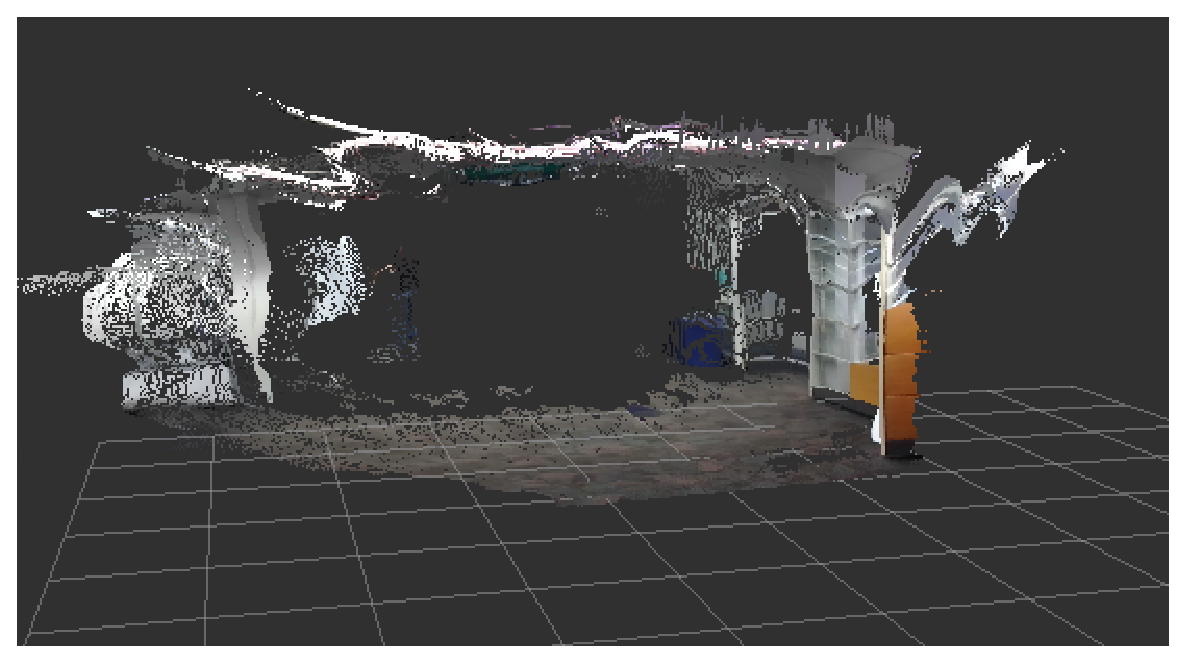
\includegraphics[width=110mm]{newpc2.eps}
\caption{Point cloud produced by the ZED drivers \label{overflow}}
\end{figure}

\begin{figure}[p!]
\centering
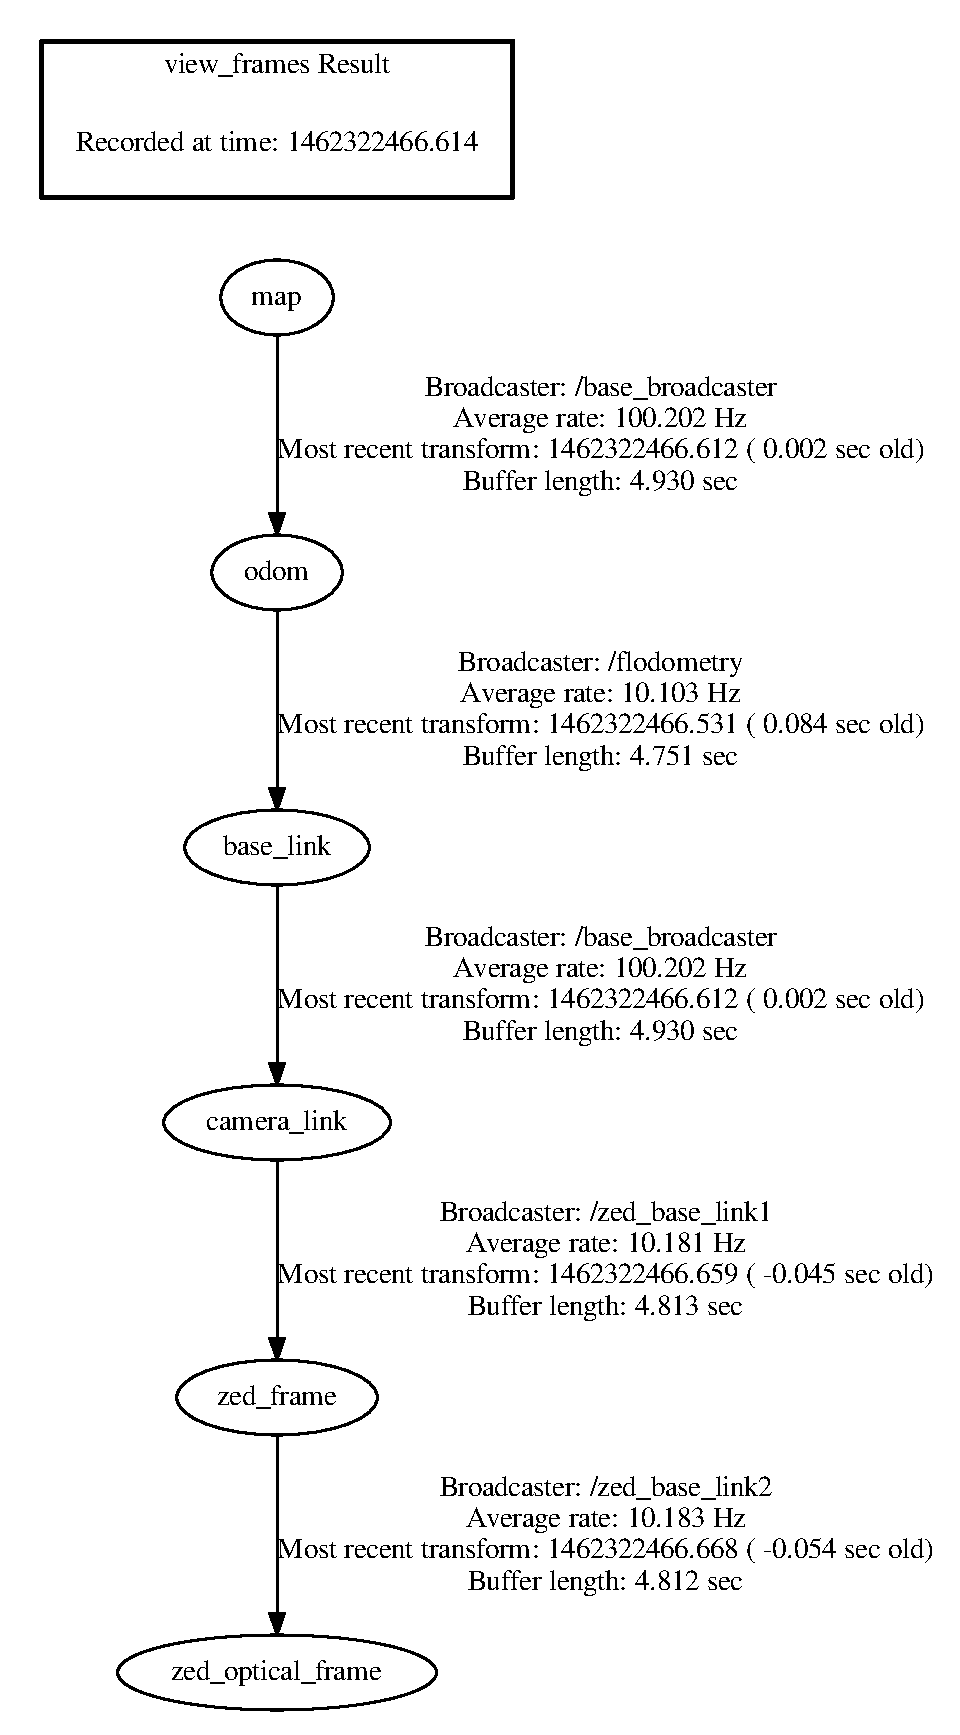
\includegraphics[width=110mm]{frames.eps}
\caption{Transformation tree of the rover}
\end{figure}

\subsection{Running the Navigation Stack}
\begin{enumerate}

\item A \texttt{map\_server} node is launched with a grayscale PGM file and a resolution value as arguments. The PGM file for level one is simply a rectangle. The dimensions are set such that the inverse of the resolution value multiplied by the number of pixels along an axis is the distance in meters. 

\item The \texttt{move\_base} node is launched with 5 YAML files as initial parameters (Figure 3). These YAML files contain the settings for the path planners and cost maps that \texttt{move\_base} will maintain. 

\item Our \texttt{navigation\_goals} node is the last to launch and contains a list of 2D coordinate goals to send to the \texttt{move\_base} node. 
\end{enumerate}

\begin{figure}
\centering
\includegraphics[width=185mm, height=85mm]{rosgraph.eps}
\caption{Node graph of the navigation stack and rover sensors. The uniboard communication node is isolated because nodes were launched using a special uniboard node designed for testing.}
\end{figure}


\section{Level Two Theory of Operation}
\subsection{Octomap}
Our initial work focused dealing with uneven ground using an \texttt{octomap\_server} node to work with a 3D occupancy grid (Figure 4). This server can read in a pre-made Octomap of the area of operation, subscribe to a point cloud topic, and subscribe to the transform corresponding to odometry data. The server uses the pre-made map and builds upon it from the point cloud input. The \texttt{octomap\_server} relies the odometry transform to iteratively update the map with the point cloud data. The server then publishes topics containing the map data that can be subscribed to for navigation. The Octomap packages do not provide costmaps like the 2D navigation stack does. Our options are to use another third party ROS library, like \texttt{humunoid\_localization}, or write our own navigation program like the team has done in the past. 

\begin{figure}[H]
\centering
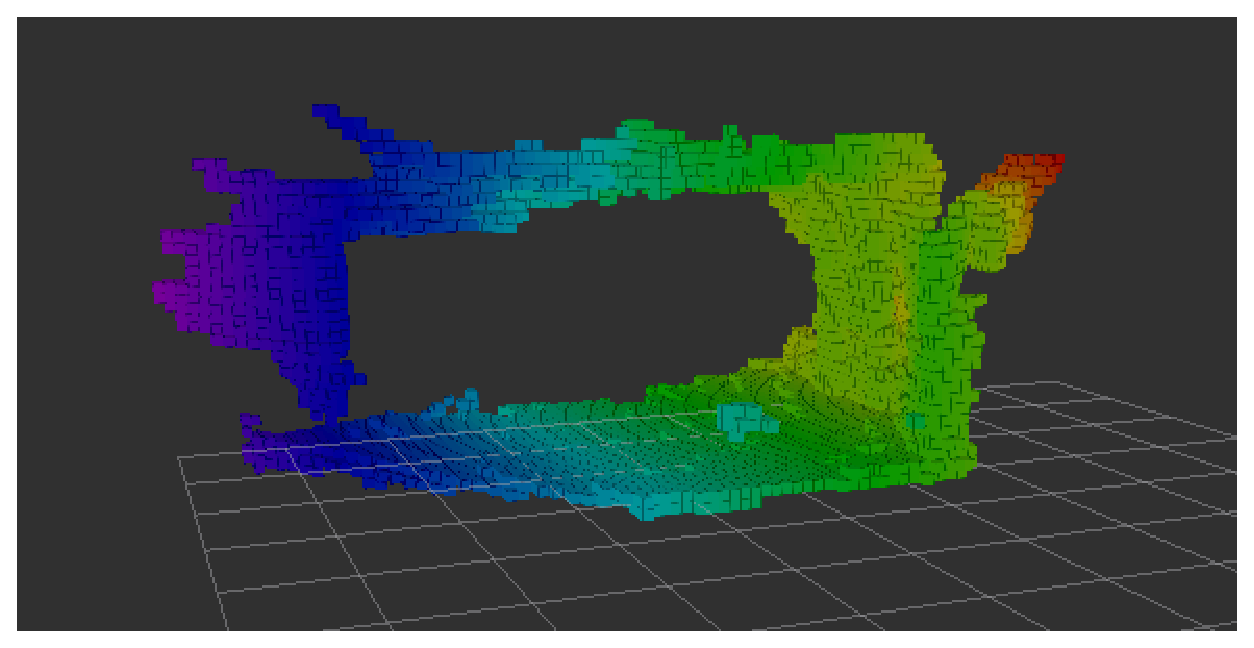
\includegraphics[width=110mm]{newoctomap.eps}
\caption{Octomap generated from the point cloud in figure 1\label{overflow}}
\end{figure}

\subsection{Generating the Seed Map}
One of the benefits of using the \texttt{octomap\_server} is that it allows for pre-existing 3D map data to be passed into the server as an argument. We can generate map data of an area to provide to the server so the rover can begin a level with knowledge of its area of operation. The server can then build on this data as the rover explores the level and maps its immediate surroundings. The \texttt{octomap\_server} requires a binary tree file type (extension .bt). To convert level data into a binary tree file we first start with Google Sketchup. With Sketchup we can select an area from the Google Maps import function, and import the region. Once imported we can make edits to the map, like known obsticles or structures to make it more accurate. Next we export the Sketchup work as a .3DS file. This file is imported into Blender. Blender allows the map to be exported as a VRML97 file.The command line program Binvox can then be used to convert this into a binvox file. Next the file is processed by an Octomap tool called binvox2bt. This converts the map to a binary tree file, the format which the \texttt{octomap\_server} can work with.


STILL NEED:

\subsection{Special Requirements to Run Software}
GPU by Nvidia 
Nvidia Cuda 
ROS Indigo
Ubuntu
Zed Stereolabs Camera
Zed SDK
Python 2.7
OpenCV 2
ROS 2D Navigation Stack
Octomap packages for ROS


STILL NEED:

Any user guides, API documentation, etc.

\section{Learning New Technology}

What web sites were helpful? (Listed in order of helpfulness.)
What, if any, reference books really helped?
Were there any people on campus that were really helpful?

\section{What You Learned}

One per team member.
What technical information did you learn?
What non-technical information did you learn?
What have you learned about project work?
What have you learned about project management?
What have you learned about working in teams?
If you could do it all over, what would you do differently?

\begin{figure}[p!]
\section{Appendix 1}
\subsection{Transform Broadcaster}
\lstinputlisting[language=C++]{transforms.cpp}
\centering
\caption{The C++ node responsible for publishing the base\_link - camera\_link transform as well as the map - odom transform. The rate setting along with the call to sleep maintain the publishing loop at approximately 100hz.}
\end{figure}

\begin{figure}[p!]
\subsection{Odom Publisher and Transform Broadcaster}
\lstinputlisting[language=Python]{flow.py}
\centering
\caption{A snippet of the Python node responsible for publishing the odom - base\_link transform as well as the \/odom topic from filtered odometry values. The odometry readings are processed in omitted functions.}
\end{figure}

\section{Appendix 2}

Appendix 2: Anything else you want to include. Photos, etc.



















\section{OLD SECTIONS: What Is Left}
\subsection{Fine Tune Odometry}
The navigation stack relies on odometry to provide good estimates of the robot's position and movement. We are testing rover movement while recording and saving odometry output to analyze the accuracy and consistency of measurements. Once this is complete the navigation stack should track our movement as best as possible. Eventually, the API for the uniboard will be extended to allow communication with the inertial measurement unit (IMU) that is onboard the rover. This will provide better information about our angle of travel. Currently the angle estimate comes from the difference in encoder values being reported. 

\subsection{Create the Bridge Between \texttt{cmd\_vel} and the PID}
\texttt{move\_base} outputs a ROS velocity data type denoted as \texttt{cmd\_vel}. Limits to the velocity and acceleration of the rover are contained within a YAML configuration files. We will make the velocity PID a subscriber to the command velocity, compute the correct values to pass to the wheels from it, and call the wheels at varied speeds to account for nonlinear movement. 

\subsection{Transition Between Team Nodes}
Both teams have been working closely the entire year and discussing how transitions should happen between states of the robot. The API for the uniboard contains two functions which may aid in this, \texttt{paused(self)}, \texttt{force\_pause(self, pause\_state)}. 
Pause returns whether or not the rover systems are currently paused. A pause would occur when the physical shutdown button on the rover is pressed, or when \texttt{force\_pause} is called. \texttt{force\_pause} switches the rover between a paused to non-paused state. The switch cannot occur if the rover was paused by the physical button. By issuing a pause when a sample is detected, the wheel commands will not be processed and the rover will halt. We could then stop navigation after the pause is issues, unpause, and allow the sample collections teams nodes to take over. 

\subsection{Returning to the Home Base}
We need to combine the nodes designed for the rover to get back to the home base with the navigation routine. We will attempt to navigate back to the home base with the planned route from the navigation stack, however the cumulative error of our odometry could make this final stretch navigation difficult if it becomes too large. Teams are allowed to place a home beacon on the starting platform that may aid in navigation back to the platform. 

\subsection{Home Beacon Options}
\begin{enumerate}
\item The team has used a simple checkerboard image on the base station in the past. We took this old code and refactored it into a ROS node and recalibrated the initial conditions to work with the ZED camera. The checkerboard identification relies on an existing OpenCV function that quickly isolates a black and white checkerboard  image from a camera frame. Using still images captured from known distances to calibrate, an estimate of distance can be made from the camera frame. Our testing found that the checkerboard can be identified consistently up to 20 meters. Using the parallelogram created by the four corners of the board, an angle estimate is produced. This angle seems accurate when the camera is still but very noisy as the camera moves. 

\item We expect to have a radio beacon working by competition. The electrical subteam has been working on the radio system to allow the rover to communicate with the base station. Their initial plan was to be able to calculate both the angle and distance from the home base to the rover. The radio was shown off at the weekly club meeting on March 6th. They reported that producing a distance estimate was not feasible but did have angle estimates working. In the demo the angles generally were estimated within a 20 degree range, but this was prone to error because it was in a small indoor space. They will have a better idea of how the radio performs once they test outdoors at greater distances. If the estimations improve once the radio is completed it may be able to be used alongside the checkerboard node to provide a more consistent angle estimate. 
\end{enumerate}

\subsection{Computation Cost and Power Usage}
We need to test that the Intel Core i5-4200U processor on the computer and 8gb of ram are sufficient enough to handle the computation capabilities we desire. With navigation nodes running we can use the \texttt{top} command and see that our nodes and ROS services are using a small portion of the system memory. This will increase when we the object recognition team adds additional camera input and processing.

Processing in all our software should be kept to a minimum due to the computationally heavy tasks the computer will run. A relatively low frame rate will be used by the ZED camera since the rover must move under 2 m/s. Using a single camera system for our vision will also decrease power usage and free up processing power without hindering the effectiveness of the navigation system. The electrical team would also like to know the amount of power that is being consumed by the computer. The rover uses a battery to provide power for the onboard systems so the additional power consumption of the computer is a concern. If the battery charge is depleted up before returning to the base station then the challenge level will not be considered complete. Fortunately, the methods used to reduce processing power will also reduce power usage. Further testing needs to be done to determine an accurate estimate of power usage.

\subsection{Level Two} We were asked to focus on level one this term since the competition date is nearing. Once we are confident in our level one ability to complete level one we will return to work on level two. The main challenge lies in the uneven ground we will face. The 2D navigation stack is not suitable for this since the path planning assumes the robot is moving on a flat surface. We plan on working with the Octomap code we have written and interfacing with the calibrated odometry data to generate three dimensional occupancy grids for level two. 

\subsection{Testing}
Our final task is to test the software on the rover. Testing has been taking place throughout the year and will continue as the software changes. The computer will be placed inside the electrical box of the rover soon which means we will need to remotely access the computer for future code changes as well as to use ROS visualization tools. We have made sure we are able to SSH into the computer to run our code, and also are able generate a hotspot on the rover and remote desktop into the machine. Future tests will be concerned with odometry tuning and measuring the accuracy of navigation over long distances. We will also test level one as a whole in a similar environment. We will test on turf with a mock base station and set up orange construction fencing to bound the area. After level one testing is completed we will begin testing level two functionality. This will include traversing more complex terrain to find samples and traveling greater distances and more Octomap testing. 

\section{Encountered Problems and Solutions}
\subsection{Working with ROS}
The way ROS code is organized and the methods of interaction between nodes is simple conceptually, however developing our code in ROS nodes was initially a challenge. We are very familiar with ROS now but found the learning curve to be steep. The provided ROS tutorials are generally helpful for learning basic concepts concerning topic communication, unfortunately many packages that provide more complex functionality give little information about how they are to be used. We have found research papers and reports on packages we are interested in, but these are often concise summaries and lack detail. ROS introductory textbooks accessible online have been very helpful.

\subsection{Working with the Octomap Packages}
Creating Octomaps from camera input was a challenge because online descriptions were unclear. When forum users or research papers discuss mapping and reference Octomap they often do not distinguish the specific ROS package in use. Since Octomap functionality is split into four packages it can be hard to determine what package is needed for the desired results. After working with the \texttt{octomap\_server} node and .bt input map files we have a much better understanding of how Octomap packages fit together. 

\subsection{Working with Another Senior Design Team}
In fall and winter terms sharing the computer between teams was an issue. Since the ZED camera drivers require an Nvidia GPU and a particular CUDA installation that we have set up on the main rover computer, most of our early vision testing required the computer. When the other team was using the computer and we wanted to work we often could not, or had to meet them to exchange the computer. This added another scheduling complication for both teams when arranging meetings. Now the computer stays stored in the Robotics lab and computer access is no longer an issue. 

\subsection{Working with the Rover Subteams}
Problems have arisen from having to meet up with other rover subteams to discuss where the team is in the project. Communication between the three teams about what sensor systems will be on the rover can be difficult. The other teams gave us the go ahead to add any sensor systems to the rover. In principle this sounded great, but since we did not have much experience with robotics at the beginning of the year it was daunting to be asked to make hardware decisions. We now assert ourselves better in team meetings than we did when the project began.

\subsection{Software and Hardware Issues}
This term we have faced issues that have arisen in working with both hardware and software. We ran into permissions difficulties between the uniboard and rover computer USB connection. We solved this by permanently changing the USB port permissions for the uniboard in \texttt{udev} to allow reading, writing and execution. Another software problem was that the computer failed to boot if the ZED camera was plugged in. We edited the boot priorities for USB devices within the BOIS to solve this. The ZED camera also failed to launch if a monitor was not plugged in. We found a VGA spoof tutorial online and asked the team to make a dummy plug for us that simulates a monitor being plugged into the computer.

We have also had some minor issues with hardware. Since the optical flow sensor does not have a housing yet it continuously disconnects while testing. Our current solution is to push in the connections and re-launch the node. This will be solved when the connections are soldered and the housing complete. A recent hardware issue that arose was a loss of communication with the uniboard that left certain parts of the rover without power. Fortunately the electrical team was able to fix this for us in an afternoon.

 We encountered a serious issue with the bash launch script we wrote to start the rover. About 40\% of the time on of the three Logitech camera launches failed due to a \texttt{device in use or busy} error. The Logitech cameras were used by the sample collection teams software, and this was an error that they had encountered when testing their code previously. We tried many different solutions to solve this launch error. One of the more promising solutions was to wait until the device was no longer busy prior to launching, but this did not work. As far as we could tell, the device was never actually busy and the error was only occurring due to us launching a group of devices simultaneously. The final solution to this problem was to simply separate every camera into it's own launch file and sleep for a period of time between calls to the files. 

\section{Conclusion}
The project has been moving along smoothly. This term has seen a shift in focus to working on 2D navigation for level one. Fortunately transforms we had developed to work with Octomap and code written to identify the home beacon all work with our 2D navigation code. We have the navigation stack running, we now need to tune our odometry and process the stack velocity commands before we begin testing complete level one functionality. We have been successful working with Octomap to map the environment in 3D and in creating maps of known environments that can work with the \texttt{octomap\_server}. We will work more with Octomap as level one testing draws to a close. Testing will continue throughout the term until we will ship the rover to Massachusetts and fly out to compete in level one of the Sample Return Robot Challenge. 

\end{document} 
